\chapter{Design Analysis and Feasibility}
\section{Safety}
Safety here



\section{Center of gravity (Fraser and Rafał)}

Seeing as the RJ100 is originally a commercial aircraft, converting it to a firefighter aircraft would result in a lot of unnecessary weight, 
for example passenger seats, kitchen and cabin bins ect.
This allows the plane to carry more retardant, meaning better performance for this specific application.
However, by removing the excess weight, the center of gravity is shifted and thus will need to be recalculated.
The RJ100 has an acceptable safe range for the center of gravity in terms of the chord length which is INSERT VALUE to INSERT VALUE.
The plane cannot fly safely if the value of the center of gravity along the x-axis of the plane is outwith this range.
The center of gravity also has to remain within this range before, during and after the ejection of retardant.

\subsection{Method of Analysis}
The process of calculating center of gravity is relatively trivial but can be time consuming if done if done by hand,
especially in this case where there are lots of components being removed, greatly altering the mass.
Using MATLAB instead of hand calculations greatly simplifies the process of changing individual values such as the mass, or the position of objects in the plane, to help achieve the safe center of gravity position. \\ 

According to \cite{baker2020engineering} the formula for the x,y and z value of the center of gravity are shown in the equation \ref{eqn:cog_formula}:

\begin{equation}
\begin{split}
  \bar{x} = \frac{\sum{ \bar{x_{i}} m_{i} }}{ \sum{ m_{i}}} \
  \bar{y} = \frac{\sum{ \bar{y_{i}} m_{i} }}{ \sum{ m_{i}}} \
  \bar{z} = \frac{\sum{ \bar{z_{i}} m_{i} }}{ \sum{ m_{i}}} \
\end{split}
\label{eqn:cog_formula}
\end{equation}

The aircraft mass and center of gravity, before excess weight removal, can effectively be represented in equation \ref{eqn:cog_formula} as a particle with known mass and position.
By representing the aircraft in this way, the center of gravity after the removal of unnecessary weight can be calculated.
The mass of the components to be removed are taken as negative, removing them from the original total mass.

\subsection{Matlab code}
Applying the method above, code was written in MATLAB to to calculate the new cg position through implementing equation \ref{eqn:cog_formula}.
This can be seen below:

\lstinputlisting{../../../code/cg_interia/cg2.m}

The data for the components to be removed were formatted into an excel file named “aircraftitems.xlsx” and then imported to be represented in the variable “Data”.
This data included each component's mass and it's center of gravity position.
These position's were taken relative to the standard aircraft axis with the origin at the nose of the aircraft.

\subsection{Consequence of result of code on design decisions}



\section{Delivery release system and  Tank Pressurisation (Anton and Fraser)}
Market analysis showed that requirements for the delivery release system (DRS) was to be able to release 3000 gallons in 8 seconds and do so with a constant, variable mass flow rate. 
The purpose of this section is to evaluate the necessary components, and operational values of these, for a system capable of meeting the design goals. The method for analysis must be simple to complete in the project timeframe whilst maintaining sufficient engineering integrity. Findings from this analysis is critical for the advancement of the design. Without proper knowledge of the components in the DRS, analysis of other areas, such as stability derivatives, cannot be carried out in full confidence. 
The following sections outlines the significant steps of the analysis of the DRS.

\subsection{Methods of Analysis}
\subsubsection{Control volume schematics}
For the purposes of the analysis the tank dimensions were set to hold the required 3000 gallons, translating to volume constraint of 13.5 $m^{2}$ . A rectangular control volume was used.

\begin{figure}[!htbp]
\centering
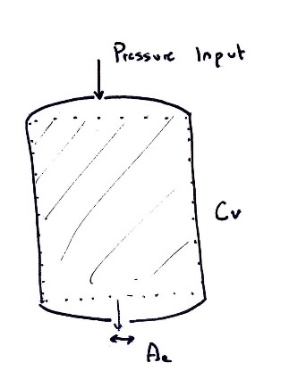
\includegraphics[width= 0.2\linewidth]{../figures/control_volume_schematic.jpg}
\caption{Control volume schematic}
\label{fig:control_volume_schematic}
\end{figure}
\FloatBarrier

Where pressure will be applied to the system via the top of the tank, Ae denoting exit area and the control volume in dashed. The control volume and exit area is largely variable and the exact dimensions are subject to change. This may be necessary due to structural or geometrical constraints.

\subsubsection{Gravity assisted drop}
This method refers to delivery purely assisted via gravity. Arguably the simplest of the methods and the cheapest. This is due to the absence of components required for pressurization, thus also allows for the largest payload. It was found that for a tank holding 3000 gallons an exit area of larger than $36 cm^{2}$  would be sufficient for an 8 second drop. 
Using the Gravity drop allows for zero control over the fluid flow rate out of the tank. Also, there could be no control over the fluid due to changes of aircraft pitch or other disturbances likely to occur in mountainous terrain. Although an increased payload could be achieved the lack of controllability outweighs this fact.

\subsubsection{Bernoulli's}
Bernoulli’s theorem allowed for a simple yet accurate way for the inclusion of pressure. By rearranging of Bernoulli’s theorem, It was possible to observe the exit velocity of the fluid as both pressure and pitch changed.


\begin{equation}
\begin{split}
  P_{top} + \frac{1}{2} \rho v^{2}_{top} + \rho g h_{top} & = P_{bot} + \frac{1}{2} \rho v^{2}_{bot} + \rho g h_{bot} \\ 
  v_{bot} & = \sqrt{\frac{2}{\rho}( \Delta P + \frac{1}{2} \rho v^{2}_{top} + \rho g \Delta h)}
\end{split}
\label{eqn:bernouli_rearanged}
\end{equation}

\begin{equation}
\begin{split}
  \dot{m} & = \rho A v_{bot}
\end{split}
\label{eqn:mass_flow}
\end{equation}

\subsection{Benchmark Simulation using Bernoulli's}
This section depicts how Bernoulli’s theorem was implemented to produce a benchmark simulation. The goal of this was to gain a base understanding of the behaviour of the DRS, benchmark values, and achieve constant mass flow. The mathematical script went through an iterative process of refinement. The final script can be seen in figure 4.3.2.

\lstinputlisting{../../../code/Pressure_Calc_Ramp.m}

To maximise our payload, it is of paramount importance that no components hold dead weight. This may appear in various scenarios, for example an unnecessarily large pressure tank for the application. Of course, the same can be said for underestimating values. 
The benchmark sim showed that all of the criteria found from market analysis was possible. Results and dimensions for the benchmark sim can be seen in figure z and z.1. A ramp input of $570 Pa/s^{2}$ was sufficient to maintain a constant mass flow rate. Meaning a maximum instantaneous input of 4560Pa. Bleed air from the engines rated at xxxxPa is more than capable of this, as well as being a resourceful solution. The retardant was released in 8 seconds meaning a total 18.24kPa was used. At this stage in the analysis that the method employed was for a simplified case. Future improvements of the simulation and results will be detailed in Section 7 Project Plan.

\subsection{Delivery release system}

The DRS is relatively simple system conceptually. A few necessary components are required, those being a piping system from the engines to a pressure tank acting as a buffer before the air is released into the pressure vessel containing our payload. Figure 4.3.3 outlines how this might look. This will be symmetric.

\begin{figure}[!htbp]
\centering
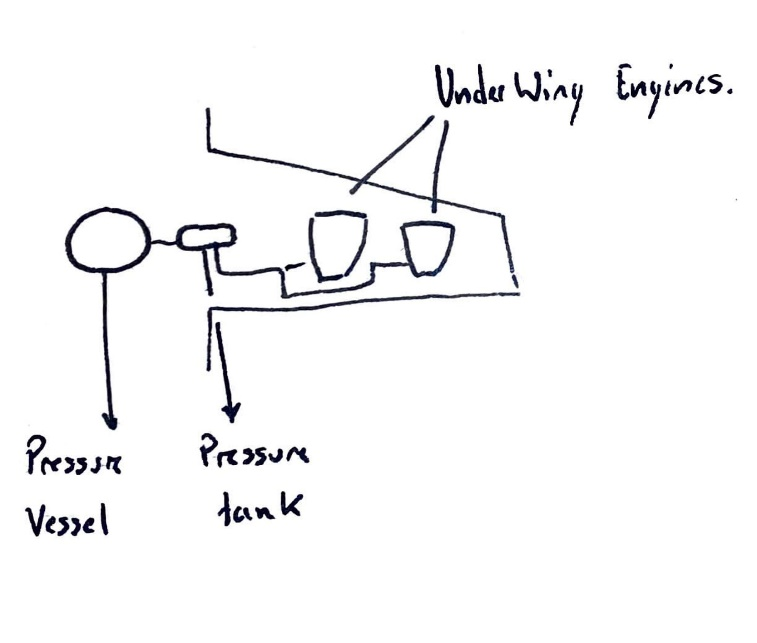
\includegraphics[width= 0.2\linewidth]{../figures/pressure_system.jpg}
\caption{pressure system}
\label{fig:pressure_system}
\end{figure}
\FloatBarrier

The pressure tank will act for as a buffer and also where the pressure controller system shall be implemented (see section 4.3.5 for controller).
Before the pressure is initially released into the pressure vessel a gap must exist between the pressure inlet and the retardant. This is to avoid the possibility of air entering regions in between the fluid causing disturbances in the flow. This is done by allowing a section of the fluid to fill into the pipes before dropping. This also allows for quicker response to pilot input.

Figure 4.3.3 depicts how this might be done. 

\begin{figure}[!htbp]
\centering
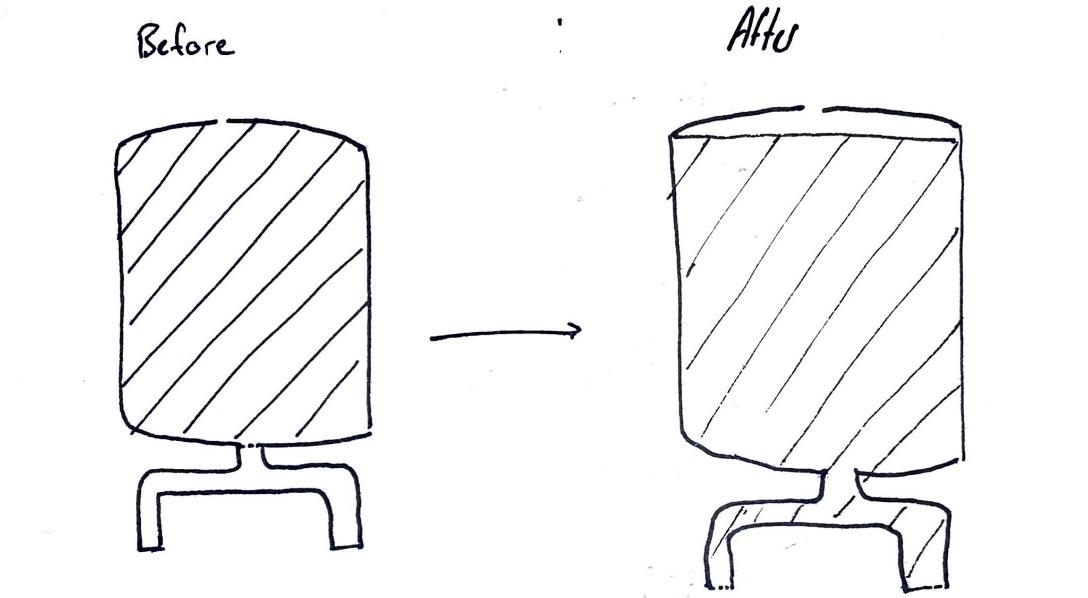
\includegraphics[width= 0.2\linewidth]{../figures/release_system_fluid_placement_control.jpg}
\caption{pressure system}
\label{fig:pressure_system}
\end{figure}
\FloatBarrier

\subsection{Controller Design}

There are two areas to consider for the controller design, the coding, and required components. The control of the fluid flow rate seen in the benchmark sim is for an extremely simplified case. It is unlikely that, given timeframe, a comprehensive code can be written ourselves. Therefor this will need to be contracted, the plans for calculating cost and other specifications of this will be covered more in section 7.
Due to modern digital controllers the weight costs of installing will be low and thus will not have a significant hinderance on payload. The exact mass of the controller is still to be decided, however examples such as the ‘Honeywell UDC2500 Universal Digital Controller’ have a quoted mass of 1.3kg [1]. Additional mechanical components will need to be fitted to the pressure tank. Power requirements are minimal.


\section{Structural Support}
Structural Support here
